%%%%%%%%%%%%%%%%%%%%%%%%%%%%%%%%%%%%%%%%%
% Beamer Presentation
% LaTeX Template
% Version 1.0 (10/11/12)
%
% This template has been downloaded from:
% http://www.LaTeXTemplates.com
%
% License:
% CC BY-NC-SA 3.0 (http://creativecommons.org/licenses/by-nc-sa/3.0/)
%
%%%%%%%%%%%%%%%%%%%%%%%%%%%%%%%%%%%%%%%%%

%----------------------------------------------------------------------------------------
%   PACKAGES AND THEMES
%----------------------------------------------------------------------------------------

\documentclass{beamer}

\mode<presentation> {

%encoding
%--------------------------------------
\usepackage[utf8]{inputenc}
\usepackage[T1]{fontenc}
%--------------------------------------

%Portuguese-specific commands
%--------------------------------------
\usepackage[portuguese]{babel}
%--------------------------------------

%Hyphenation rules
%--------------------------------------
\usepackage{hyphenat}
\hyphenation{mate-mática recu-perar}
%--------------------------------------

\bibliographystyle{plain}



% The Beamer class comes with a number of default slide themes
% which change the colors and layouts of slides. Below this is a list
% of all the themes, uncomment each in turn to see what they look like.

%\usetheme{default}
%\usetheme{AnnArbor}
%\usetheme{Antibes}
%\usetheme{Bergen}
\usetheme{Berkeley}
%\usetheme{Berlin}
%\usetheme{Boadilla}
%\usetheme{CambridgeUS}
%\usetheme{Copenhagen}
%\usetheme{Darmstadt}
%\usetheme{Dresden}
%\usetheme{Frankfurt}
%\usetheme{Goettingen}
%\usetheme{Hannover}
%\usetheme{Ilmenau}
%\usetheme{JuanLesPins}
%\usetheme{Luebeck}
%\usetheme{Madrid}
%\usetheme{Malmoe}
%\usetheme{Marburg}
%\usetheme{Montpellier}
%\usetheme{PaloAlto}
%\usetheme{Pittsburgh}
%\usetheme{Rochester}
%\usetheme{Singapore}
%\usetheme{Szeged}
%\usetheme{Warsaw}

% As well as themes, the Beamer class has a number of color themes
% for any slide theme. Uncomment each of these in turn to see how it
% changes the colors of your current slide theme.

%\usecolortheme{albatross}
%\usecolortheme{beaver}
%\usecolortheme{beetle}
%\usecolortheme{crane}
%\usecolortheme{dolphin}
%\usecolortheme{dove}
%\usecolortheme{fly}
%\usecolortheme{lily}
%\usecolortheme{orchid}
%\usecolortheme{rose}
%\usecolortheme{seagull}
%\usecolortheme{seahorse}
%\usecolortheme{whale}
%\usecolortheme{wolverine}

%\setbeamertemplate{footline} % To remove the footer line in all slides uncomment this line
%\setbeamertemplate{footline}[page number] % To replace the footer line in all slides with a simple slide count uncomment this line

%\setbeamertemplate{navigation symbols}{} % To remove the navigation symbols from the bottom of all slides uncomment this line
}

\usepackage{graphicx} % Allows including images
\usepackage{booktabs} % Allows the use of \toprule, \midrule and \bottomrule in tables

%----------------------------------------------------------------------------------------
%   TITLE PAGE
%----------------------------------------------------------------------------------------

\title[Firewall]{Redes de Computadores 2 - Firewall} % The short title appears at the bottom of every slide, the full title is only on the title page

\author{Gustavo Yudi Bientinezi Matsuzake} % Your name
\institute[UTFPR] % Your institution as it will appear on the bottom of every slide, may be shorthand to save space
{
Universidade Tecnológica Federal do Paraná\\ % Your institution for the title page
Profº Fabiano Scriptore de Carvalho \\
\medskip
\textit{yudi.matsuzake@gmail.com} % Your email address
\url{https://github.com/yudi-matsuzake/firewall-apresentacao}
}
\date{\today} % Date, can be changed to a custom date

\begin{document}

\begin{frame}
\titlepage % Print the title page as the first slide
\end{frame}

\begin{frame}
\frametitle{Sumário} % Table of contents slide, comment this block out to remove it
\tableofcontents % Throughout your presentation, if you choose to use \section{} and \subsection{} commands, these will automatically be printed on this slide as an overview of your presentation
\end{frame}

%----------------------------------------------------------------------------------------
%   PRESENTATION SLIDES
%----------------------------------------------------------------------------------------

\section{Introdução} 

\subsection{O que é?} % A subsection can be created just before a set of slides with a common theme to further break down your presentation into chunks

%-----------------------------------------------
\begin{frame}
	\frametitle{Denifição}

	\begin{itemize}
		\item Em computação, um firewall é um sistema de segurança de redes de computadores;
		\item Note que é um SISTEMA (não apenas software, hardware ou um muro mesmo);
		\item SIM, os três podem ser um sistema de firewall em computação (até o muro)!
	\end{itemize}

\end{frame}

%------------------------------------------------

\subsection{Onde posso encontrar firewalls?}
\begin{frame}
	%NETGATE
	\begin{figure}
		\centering
		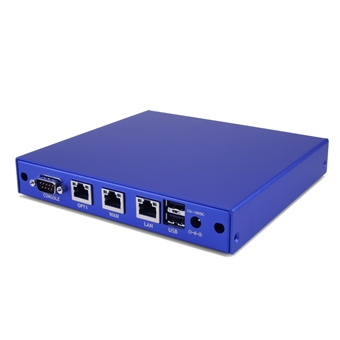
\includegraphics[height=0.3\textheight]{imagens/netgate.jpg}
		\caption{Netgate}
	\end{figure}
	
	%DELL
	\begin{figure}
		\centering
		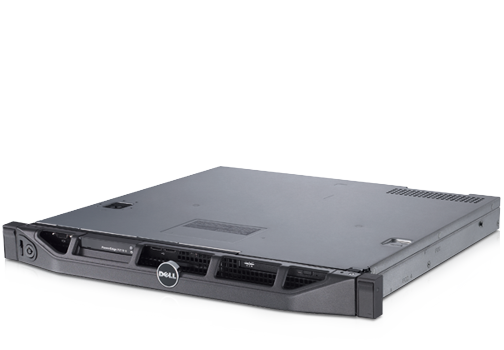
\includegraphics[height=0.3\textheight]{imagens/dell.png}
		\caption{Dell}
	\end{figure}

\end{frame}

%------------------------------------------------

\subsection{Analogia do castelo}




\section{História}

\begin{frame}
	\frametitle{O começo \cite{history}} 

	\begin{itemize}
		\item A internet era suportada por uma comunidade pequena;
		\item Era formada de usuários que valorizavam a liberdade de compartilhar e colaboração;
		\item Em 1988 Clifford Stoll descobriu espiões russos zoando com seu sistema \cite{stoll};
		\begin{itemize}
			\item{Criaram uma "cadeia" para o hacker;}
			\item{Deixaram ele pensar que ele tinha realmente invadido;}
			\item{Estudaram seus ataques e seus métodos;}
			\item{Daí tomaram medidas administrativas na rede.}
		\end{itemize}
		\item Uma curiosidade interessante da história dos firewalls é que seu desenvolvimento foi coincidindo em métodos cada vez mais "altos" nas camadas de protocolos da camada OSI.
	\end{itemize}
\end{frame}


\section{Tipos de firewall}

\begin{frame}
	\frametitle{Tipos de firewall}
	\begin{itemize}
		\item Primeira geração: Filtros de pacote (Filtros "\textit{Stateless}");

		\item Segunda geração: Filtros "\textit{Stateful}";

		\item Terceira geração: Camada de aplicação.
	\end{itemize}
\end{frame}


%----------------------------
%FUNCIONAMENTO
%QUAIS SÃO OS ATRIBUTOS DAS POLÍTICAS?
%Quais camadas?
%EXEMPLOS

\subsection{Filtros de pacote (stateless)}

\begin{frame}
	\frametitle{Funcionamento}
	\begin{itemize}
		\item Seu funcionamento é baseado na filtragem de pacotes; (ah, vá!)
		\item Seu funcionamento é simples:
		\begin{itemize}
			\item Se o pacote casar com as políticas do firewall:
				\begin{itemize}
					\item O pacote entra na rede na maior tranquilidade;
				\end{itemize}
			\item Se o pacote não casar com as políticas do firewall:
				\begin{itemize}
					\item O pacote é descartado;
				\end{itemize}
		\end{itemize}
	\end{itemize}
\end{frame}

\begin{frame}
	\frametitle{Políticas}
	\begin{itemize}
		\item Esse tipo de firewall só verifica a informação do pacote em si;
		\item i.e. o firewall não guarda a informação do status da conexão;
		\item Geralmente atributos verificados são:
			\begin{itemize}
				\item IP de origem e IP de destino
				\item O protocolo (UDP e TCP)
				\item A porta
			\end{itemize}
	\end{itemize}
\end{frame}

\begin{frame}
	\frametitle{Modelo OSI}

	\begin{itemize}
		\item O firewall stateless verifica informações das camadas física, enlace, rede e um pouquinho da camada de transporte;
	\end{itemize}

\end{frame}

\begin{frame}
	\frametitle{Exemplos}
	\begin{itemize}
		\item ACL - \textit{Access Control List}
		\item iptables \footnote{O iptables por si só não é um firewall stateful. Mas o iptables se torna uma ferramenta muito fácil de se \textit{scriptar} um firewall stateful};
	\end{itemize}
\end{frame}

\subsection{Filtros de estado de conexão (stateful)}

\begin{frame}
	\frametitle{Funcionamento}
	\begin{itemize}
		\item Um firewall stateful é qualquer firewall que consegue fazer uma Inspeção de Pacotes Stateful \footnote{Traduzido livremente de SPI - Stateful Packet Inspection};
		\item Firewalls Stateful trabalham fortemente na camada de transporte, pois guardam o estado das conexões TCP e UDP;
		\item Guardando os estados das conexões, esses firewalls conseguem gerar atributos significantes de cada conexão e gerenciá-las;
		\item Eles também tem um banco de dados de possíveis sessões de ataques, se essa sessão não é permitida o pacote é dropado;
		\item Sistema para não encher a memória de sessões apenas inicializadas apartir do three-way handshake;
		\item Problema keepalive;
		\item A maioria dos firewalls mais modernos são statefull;
	\end{itemize}
\end{frame}


\subsection{Camada de aplicaçao}

\begin{frame}
	\frametitle{Funcionamento}
	\begin{itemize}
		\item São chamados de Firewalls da Próxima Geração (NGFW\footnote{Next-generation Firewall});
		\item Trabalham na camada de aplicação e "entendem" como os protocolos dessa camada funcionam (e.g FTP, DNS, HTTP);
		\item Inspecionam profundamente os pacotes e seções DPI\footnote{Tradução livre de \textit{deep packet inspection}};
	\end{itemize}
\end{frame}

\begin{frame}
	\frametitle{Funcionalidades extendidas}
	As três funcionalidades que DEVEM ter em um NGFW por causa do DPI e não tem em um stateful firewall é:
	\begin{enumerate}[i]
		\item Sistema de Prevenção de Intrusão (IPS\footnote{Intrusion Prevention System});
		\item Integração a Identificação do Usuário (UII\footnote{User Identity Integration});
		\item Firewall de Aplicação Web (WAF \footnote{Web Application Firewall}).
	\end{enumerate}
\end{frame}


%------------------------------------------------

\begin{frame}
\frametitle{Blocks of Highlighted Text}
\begin{block}{Block 1}
Lorem ipsum dolor sit amet, consectetur adipiscing elit. Integer lectus nisl, ultricies in feugiat rutrum, porttitor sit amet augue. Aliquam ut tortor mauris. Sed volutpat ante purus, quis accumsan dolor.
\end{block}

\begin{block}{Block 2}
Pellentesque sed tellus purus. Class aptent taciti sociosqu ad litora torquent per conubia nostra, per inceptos himenaeos. Vestibulum quis magna at risus dictum tempor eu vitae velit.
\end{block}

\begin{block}{Block 3}
Suspendisse tincidunt sagittis gravida. Curabitur condimentum, enim sed venenatis rutrum, ipsum neque consectetur orci, sed blandit justo nisi ac lacus.
\end{block}
\end{frame}

%------------------------------------------------

\begin{frame}
\frametitle{Multiple Columns}
\begin{columns}[c] % The "c" option specifies centered vertical alignment while the "t" option is used for top vertical alignment

\column{.45\textwidth} % Left column and width
\textbf{Heading}
\begin{enumerate}
\item Statement
\item Explanation
\item Example
\end{enumerate}

\column{.5\textwidth} % Right column and width
Lorem ipsum dolor sit amet, consectetur adipiscing elit. Integer lectus nisl, ultricies in feugiat rutrum, porttitor sit amet augue. Aliquam ut tortor mauris. Sed volutpat ante purus, quis accumsan dolor.

\end{columns}
\end{frame}

%------------------------------------------------
\section{Second Section}
%------------------------------------------------

\begin{frame}
\frametitle{Table}
\begin{table}
\begin{tabular}{l l l}
\toprule
\textbf{Treatments} & \textbf{Response 1} & \textbf{Response 2}\\
\midrule
Treatment 1 & 0.0003262 & 0.562 \\
Treatment 2 & 0.0015681 & 0.910 \\
Treatment 3 & 0.0009271 & 0.296 \\
\bottomrule
\end{tabular}
\caption{Table caption}
\end{table}
\end{frame}

%------------------------------------------------

\begin{frame}
\frametitle{Theorem}
\begin{theorem}[Mass--energy equivalence]
$E = mc^2$
\end{theorem}
\end{frame}

%------------------------------------------------

\begin{frame}[fragile] % Need to use the fragile option when verbatim is used in the slide
\frametitle{Verbatim}
\begin{example}[Theorem Slide Code]
\begin{verbatim}
\begin{frame}
\frametitle{Theorem}
\begin{theorem}[Mass--energy equivalence]
$E = mc^2$
\end{theorem}
\end{frame}\end{verbatim}
\end{example}
\end{frame}

%----------------------------------------------

\begin{frame}
\frametitle{Figure}
Uncomment the code on this slide to include your own image from the same directory as the template .TeX file.
\begin{figure}
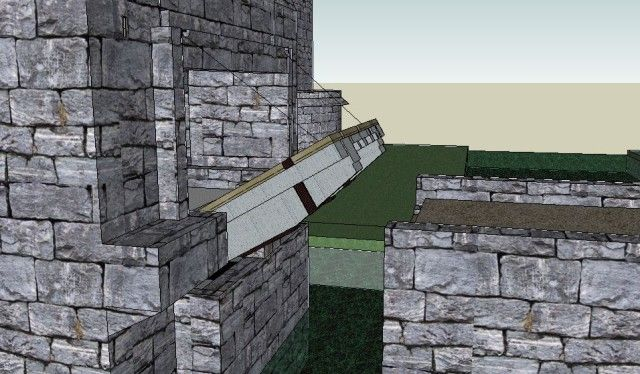
\includegraphics[width=0.8\linewidth]{imagens/castelo-ponte.jpg}
\end{figure}
\end{frame}

%------------------------------------------------

\begin{frame}[fragile] % Need to use the fragile option when verbatim is used in the slide
\frametitle{Citation}
An example of the \verb|\cite| command to cite within the presentation:\\~

This statement requires citation \cite{talal}.
\end{frame}

%------------------------------------------------

\begin{frame}
\frametitle{References}
%\footnotesize{
%\begin{thebibliography}{99} % Beamer does not support BibTeX so references must be inserted manually as below
%\bibitem[Smith, 2012]{p1} John Smith (2012)
%\newblock Title of the publication
%\newblock \emph{Journal Name} 12(3), 45 -- 678.
%\end{thebibliography}
%}
\bibliography{apresentacao}
\end{frame}

%------------------------------------------------

\section{FIM}
\begin{frame}
\frametitle{Acabou :(}
\centerline{Dúvidas?}

\titlepage
\end{frame}

%----------------------------------------------------------------------------------------

\end{document}
